% THIS IS SIGPROC-SP.TEX - VERSION 3.1
% WORKS WITH V3.2SP OF ACM_PROC_ARTICLE-SP.CLS
% APRIL 2009
%
% It is an example file showing how to use the 'acm_proc_article-sp.cls' V3.2SP
% LaTeX2e document class file for Conference Proceedings submissions.
% ----------------------------------------------------------------------------------------------------------------
% This .tex file (and associated .cls V3.2SP) *DOES NOT* produce:
%       1) The Permission Statement
%       2) The Conference (location) Info information
%       3) The Copyright Line with ACM data
%       4) Page numbering
% ---------------------------------------------------------------------------------------------------------------
% It is an example which *does* use the .bib file (from which the .bbl file
% is produced).
% REMEMBER HOWEVER: After having produced the .bbl file,
% and prior to final submission,
% you need to 'insert'  your .bbl file into your source .tex file so as to provide
% ONE 'self-contained' source file.
%
% Questions regarding SIGS should be sent to
% Adrienne Griscti ---> griscti@acm.org
%
% Questions/suggestions regarding the guidelines, .tex and .cls files, etc. to
% Gerald Murray ---> murray@hq.acm.org
%
% For tracking purposes - this is V3.1SP - APRIL 2009
\documentclass{acm_proc_article-sp}
\usepackage{graphicx}

\begin{document}

\title{Improving Live Migration: is it even worth it?}
% You need the command \numberofauthors to handle the 'placement
% and alignment' of the authors beneath the title.
%
% For aesthetic reasons, we recommend 'three authors at a time'
% i.e. three 'name/affiliation blocks' be placed beneath the title.
%
% NOTE: You are NOT restricted in how many 'rows' of
% "name/affiliations" may appear. We just ask that you restrict
% the number of 'columns' to three.
%
% Because of the available 'opening page real-estate'
% we ask you to refrain from putting more than six authors
% (two rows with three columns) beneath the article title.
% More than six makes the first-page appear very cluttered indeed.
%
% Use the \alignauthor commands to handle the names
% and affiliations for an 'aesthetic maximum' of six authors.
% Add names, affiliations, addresses for
% the seventh etc. author(s) as the argument for the
% \additionalauthors command.
% These 'additional authors' will be output/set for you
% without further effort on your part as the last section in
% the body of your article BEFORE References or any Appendices.

\numberofauthors{2} %  in this sample file, there are a *total*
% of EIGHT authors. SIX appear on the 'first-page' (for formatting
% reasons) and the remaining two appear in the \additionalauthors section.
%
\author{
% You can go ahead and credit any number of authors here,
% e.g. one 'row of three' or two rows (consisting of one row of three
% and a second row of one, two or three).
%
% The command \alignauthor (no curly braces needed) should
% precede each author name, affiliation/snail-mail address and
% e-mail address. Additionally, tag each line of
% affiliation/address with \affaddr, and tag the
% e-mail address with \email.
%
% 1st. author
\alignauthor
Zachary Estrada
\email zestrad2@illinois.edu
\alignauthor
Furquan Shaikh
\email fmshaik2@illinois.edu
}

\maketitle
\begin{abstract}
Virtualization technology is ubiquitous in most of today's datacenters and is an enabling technology for Infrastructure-as-a-Service Cloud Computing.  As the size of VM farms grows, concerns about the scalability of managing this infrastructure is growing.  Live migration techniques offer large flexibility gains at the cost of increased network traffic.  One solution to reduce this traffic involves exploiting the redundancy of data across virtual machines by migrating groups of similar virtual machines.  For this to be a worthwhile endeavor, we must first understand the nature of this redundancy.  The goal of this study is to investigate some possible use cases and determine the amount of memory redundancy that exists across VMs for these cases.  We develop a platform for evaluating this redundnacy and then utilize it to gain insight into the level of redundancy that can be exploited in these systems.
\end{abstract}

% A category with the (minimum) three required fields
%\category{H.4}{Information Systems Applications}{Miscellaneous}
%A category including the fourth, optional field follows...
%\category{D.2.8}{Software Engineering}{Metrics}[complexity measures, performance measures]
\setlength{\parindent}{0.5cm}
\section{Introduction}
Virtualization has become one of the most important technologies in today's era. It plays a crucial role in many distributed systems and services. It also forms the fundamental block in cloud computing solutions, such as Amazon EC2 \cite{ec2} and Windows Azure\cite{azure}. The reason that virtualization is widely used in such systems is that it makes better utilization of resources and reduces the cost by allowing multiple operating systems to run concurrently on the same physical infrastructure. Multiple operating systems running in their own virtual machines share the hardware resources, while ensuring high availability for the user applications \cite{virt_app}.
\par
\begin{figure}[htbp]
\centering
        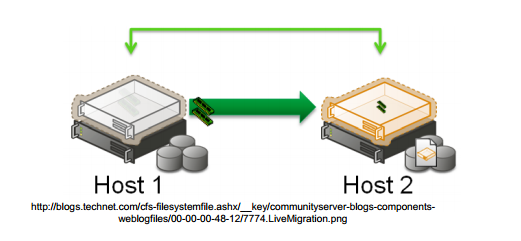
\includegraphics[height=4cm,width=9cm]{live_migration.png}
    \caption{Live Migration}
    \label{fig:live_migration}
\end{figure}
\indent With the increase in size of VM farms, scalability and manageability become a major concern. In order to solve these problems, live migration of a VM was  designed as a powerful tool. Live migration allows VMs to be reorganized for improving reachability, fault-tolerance as well as load balancing within VM farms. The basic idea of live migration is depicted in Figure \ref{fig:live_migration} \cite{live_migration}.
\par
\begin{figure}
\centering
        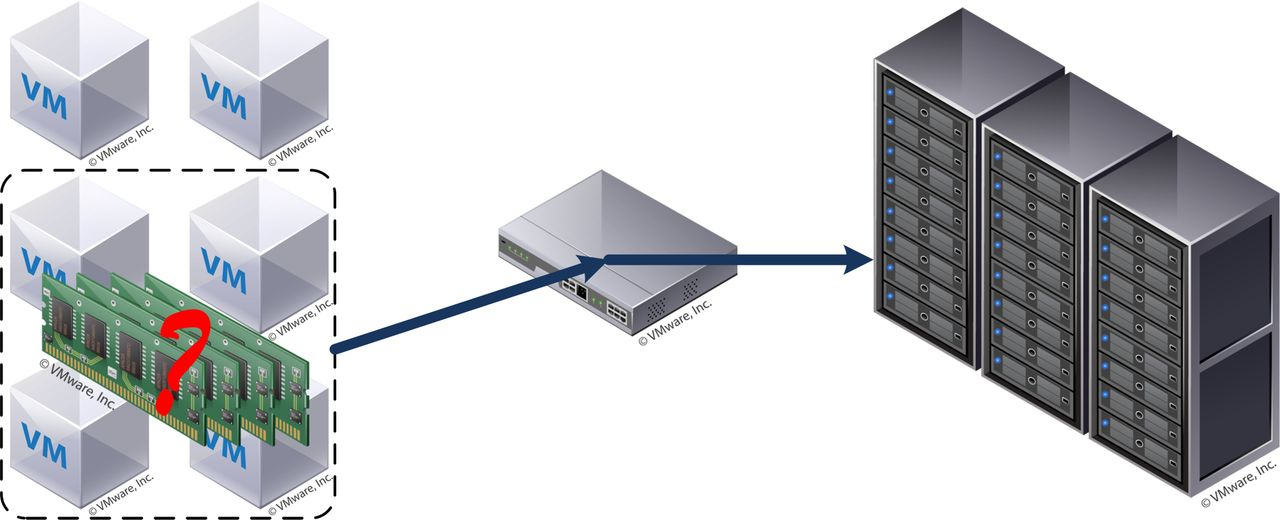
\includegraphics[height=8cm,width=9cm]{gang_migration.jpg}
    \caption{Live Gang Migration}
    \label{fig:gang_migration}
\end{figure}
However, it is generally observed that a group of multiple VMs co-ordinate with each other in order to provide services to clients. For example, in a Map-Reduce kind of workload, the mappers and reducers are spread over a set of different VMs and all these jobs co-ordinate with each other to accomplish the goal of the user. Also, in web-server kind of environments, the web-server, database server and other servers are spread over a set of VMs in order to provide service to client requests. Thus, in order to ensure maximum performance and lower downtime for processing client requests, it is necessary to perform gang live migration of all co-ordinating VMs rather than a single live migration of individual VMs. The concept of gang live migration is shown in Figure \ref{fig:gang_migration}.
\par
Though live migration proves to be a powerful tool in increasing the manageability of the VM farms, it comes at the cost of increased network traffic. One solution to reduce this traffic is to exploit the redundancy of data across virtual machines by migrating groups of similar virtual machines. Theoretically, there exists redundant memory content across VMs in the form of kernel code, kernel static data, application libraries as well as application binaries. However, in order to ensure that the whole process of exploiting redundancy for gang live migration is worthwhile, we need to first understand the nature of this redundancy.
\par
This project aims at investigating deeper into different practical use cases and determine the amount of memory redundancy that exists across VMs for these cases. The observations and conclusions presented in this paper can be used as a guideline in deciding if it is worthwhile to invest in a distributed solution for exploiting memory redundancy for group live migration.
\par

\section{Redundancy Evaluation Architecture}


\section{Optimistic Upper Bounds}
Before we proceed with applied use cases, we decided to get an upper bound for redundancy by testing a subset of ``ideal'' situations.

%Here, we compare two basic cases. On the left, we have one cloud image that is instantiated multiple times. On the right, we test VMs of different operating systems against each other. The half above the diagonal does not include zero pages and the lower half includes zero pages. As can be expected, not much redundancy exists across different OS versions (though this may change with real applications). All VMs have 1GB of memory.


\section{Stability Over Time}
Folding at home, surprising that it was stable until...

\section{Client-Server}

\section{Hadoop}

\section{Stability Over Time}

\section{Conclusions}

\bibliographystyle{abbrv}
\bibliography{cs598mcc_paper}

\end{document}
